\chapter{Preliminares}

En este capítulo se presentan los conceptos y fundamentos teóricos necesarios para comprender los temas tratados en este trabajo. 
Se abordarán las bases de la tecnología \textit{blockchain} y las infraestructuras de clave pública (\textit{PKI}), destacando su 
relevancia y características principales.

\section{Criptografía asimétrica}

La criptografía asimétrica, también conocida como criptografía de clave pública, es un paradigma de cifrado que utiliza un par de claves: una pública, que 
puede ser compartida libremente, y una privada, que debe mantenerse en secreto. Este esquema permite garantizar la confidencialidad, integridad y 
autenticación en sistemas de comunicación modernos.

El verdadero despegue de esta técnica llegó en 1977 con la creación del algoritmo RSA \cite{rivest1978method}, desarrollado por Ronald Rivest, Adi Shamir y Leonard Adleman. 
Este sistema utiliza un par de claves matemáticamente relacionadas: una clave pública, que puede ser compartida libremente, y una clave privada, que debe 
mantenerse en secreto. La clave pública cifra el mensaje, mientras que la clave privada se utiliza para descifrarlo. Este enfoque resuelve el problema 
de la distribución segura de claves y hace posible la autenticación y el intercambio seguro de información en entornos inseguros como Internet.

La criptografía de clave pública surgió como una solución a dos problemas fundamentales de la criptografía simétrica:
\begin{itemize}
  \item \textbf{Distribución de claves:} En la criptografía simétrica, la distribución de claves requiere que las partes que desean comunicarse ya compartan una clave secreta o dependan de un Centro de Distribución de Claves (KDC, por sus siglas en inglés). Según Whitfield Diffie, uno de los descubridores de la criptografía de clave pública, este enfoque comprometía la esencia misma de la criptografía: mantener el secreto total de las comunicaciones. Él argumentaba: "¿De qué servirían sistemas criptográficos impenetrables si sus usuarios debieran compartir sus claves con un KDC que podría ser comprometido?" \cite{diffie1976new}
  \item \textbf{Firmas digitales:} La criptografía debía evolucionar para ser utilizada en aplicaciones comerciales y privadas, además de las militares. Esto requería un mecanismo equivalente a las firmas en documentos en papel, que garantizara de manera verificable que un mensaje digital provenía de una persona específica.
\end{itemize}

A continuación, se describen algunos términos fundamentales relacionados con este tipo de criptografía:

\begin{itemize}
  \item \textbf{Claves asimétricas}: Un par de claves relacionadas (clave pública y clave privada) que se utilizan para operaciones complementarias como el cifrado/descifrado o la generación/verificación de firmas.
  \item \textbf{Certificado de clave pública}: Un documento digital emitido y firmado por una Autoridad de Certificación (CA) que vincula el nombre de un usuario con su clave pública y confirma que solo el titular tiene acceso a la clave privada correspondiente.
  \item \textbf{Algoritmo criptográfico de clave pública}: Un algoritmo que emplea un par de claves asimétricas. La derivación de la clave privada a partir de la pública debe ser computacionalmente inviable.
  \item \textbf{Infraestructura de Clave Pública}: Conjunto de políticas, procesos, servidores, software y equipos utilizados para administrar certificados digitales y pares de claves públicas/privadas. Esto incluye la emisión, el mantenimiento y la revocación de certificados.
  \item \textbf{Llaves pública y privada}: Estas forman un par de llaves seleccionadas para que si una se utiliza para cifrar, la otra pueda descifrar. Las transformaciones realizadas dependen de cuál de las llaves (pública o privada) se utiliza como entrada.
  \item \textbf{Texto cifrado (Ciphertext)}: Es el mensaje cifrado que se produce como salida del algoritmo. Depende del mensaje original (plaintext) y de la llave utilizada. Para un mismo mensaje, dos llaves diferentes producen textos cifrados diferentes.
  \item \textbf{Algoritmo de descifrado}: Es el proceso que toma el texto cifrado y la llave correspondiente para devolver el mensaje original.
\end{itemize}

\begin{figure}[!htbp]
    \centering
    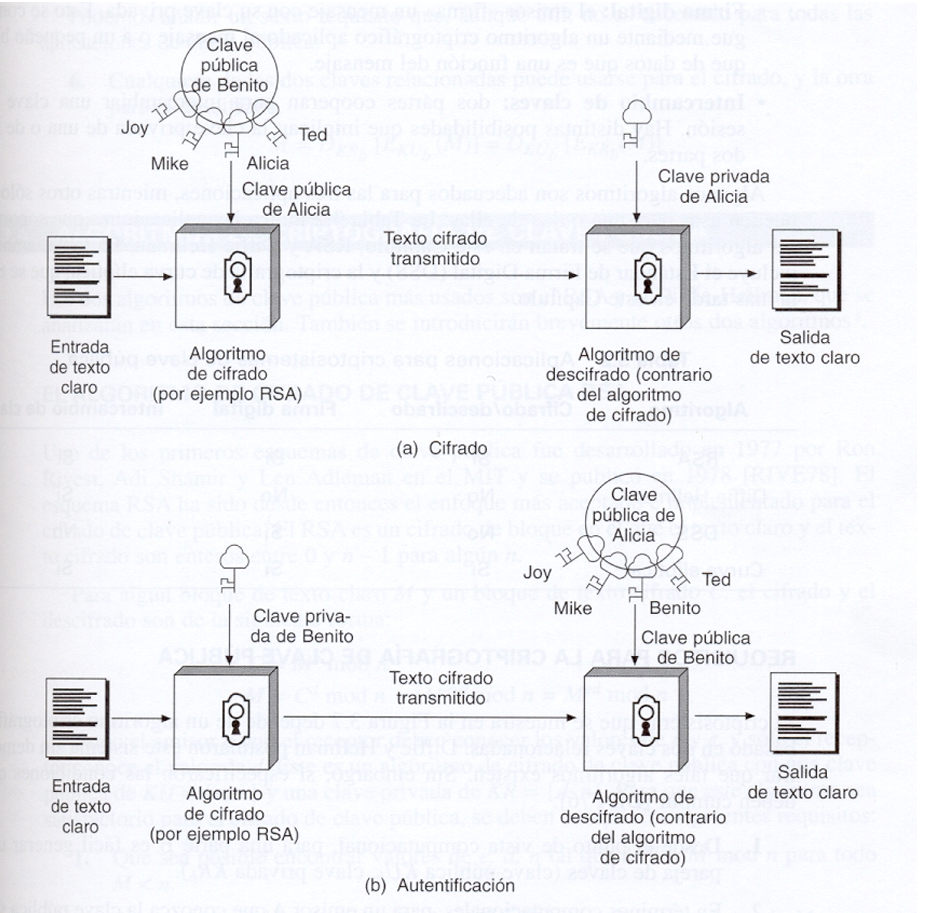
\includegraphics[width=0.7\textwidth]{./Graphics/cifrado_esquema.png}
    \caption{\scriptsize Esquema de uso de los algoritmos de cifrado asimétrico.}
    \label{fig:Cipher}
\end{figure}

Pasos esenciales del cifrado de clave pública
\begin{itemize}
  \item \textbf{Generación de llaves}: Cada usuario genera un par de llaves para cifrar y descifrar mensajes.
  \item \textbf{Distribución de la llave pública}: Cada usuario coloca una de las llaves (la pública) en un registro accesible. La llave privada se mantiene secreta.
  \item \textbf{Proceso de cifrado}:
  \begin{itemize}
    \item Si Bob desea enviar un mensaje confidencial a Alice, utiliza la llave pública de Alice para cifrarlo.
    \item Al recibir el mensaje, Alice lo descifra utilizando su llave privada.
  \end{itemize}  
  \item \textbf{Confidencialidad asegurada}:
  \begin{itemize}
    \item Todos los participantes tienen acceso a las llaves públicas de otros usuarios.
    \item Las llaves privadas nunca necesitan ser compartidas.
    \item Mientras una llave privada esté protegida, la comunicación permanece segura.
  \end{itemize}  
  \item \textbf{Rotación de llaves}: En caso de ser necesario, cualquier usuario puede generar una nueva llave privada y publicar la nueva llave pública para reemplazar la anterior.
\end{itemize}  
Este enfoque asegura:
\begin{itemize}
  \item Confidencialidad: Solo el receptor (Alice) puede descifrar el mensaje.
  \item Gestión sencilla de llaves: No es necesario compartir o enviar la llave privada, reduciendo el riesgo de compromiso.
\end{itemize}

Un criptosistema con estas características no es suficientemente seguro, ya que sigue siendo vulnerable a ataques de tipo \textit{\textbf{Man-in-the-Middle}} (como se muestra en la figura \ref{fig:MIM}) y a la suplantación de identidad. Por ejemplo, si un usuario \textbf{D} publica su clave pública \textbf{PUd} haciéndola pasar por la clave de otro usuario \textbf{B}, cualquier persona que intente comunicarse con \textbf{B} podría utilizar \textbf{PUd} para cifrar su mensaje, creyendo erróneamente que está enviándolo de forma segura a \textbf{B}. En este caso, si \textbf{D} intercepta el mensaje, podrá descifrarlo fácilmente con su clave privada, comprometiendo así la confidencialidad de la comunicación.

\begin{figure}[!htbp]
    \centering
    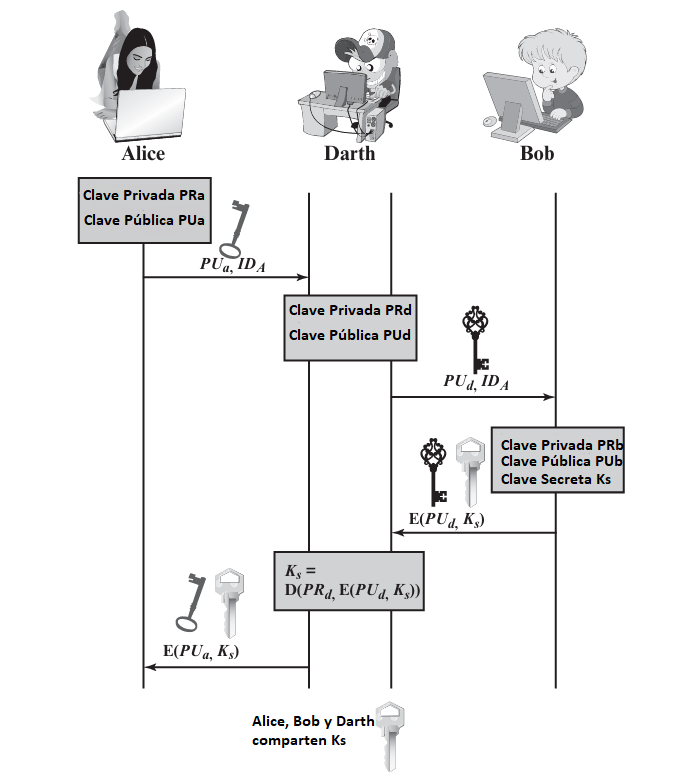
\includegraphics[width=0.7\textwidth]{./Graphics/MIM.png}
    \caption{\scriptsize Ataque \textit{Man-in-the-Middle}.}
    \label{fig:MIM}
\end{figure}

Para mitigar riesgos de seguridad como los mencionados, se emplean los \textbf{certificados digitales}, que actúan como una prueba firmada que garantiza que una identidad es realmente quien dice ser. 
La emisión de estos certificados recae en una autoridad de confianza conocida como \textbf{CA} (por sus siglas en inglés, \textit{Certification Authority}). 
Esta autoridad debe contar con su propio certificado que la valide como una \textbf{CA} confiable, emitido por otra \textbf{CA} o, en última instancia, por una autoridad raíz. 
Toda esta información debe estar reflejada en el certificado, creando así una red de confianza transparente y auditable.

\section{Infraestructura de Clave Pública}

La infraestructura de clave pública, como se mencionó anteriormente, es el conjunto de entidades que incluyen software, políticas, procedimientos, hardware y personas, que participan en la gestión de la emisión, verificación y revocación de certificados digitales. Su principal objetivo es permitir la adquisición de claves públicas de manera segura, conveniente y eficiente.

\subsection{Componentes principales de una PKI}

Una \textbf{PKI} se compone de varios elementos fundamentales, descritos a continuación:

\begin{itemize}
    \item \textbf{Entidad final (End Entity)}: Término genérico para designar a los usuarios finales, dispositivos (por ejemplo, servidores, enrutadores) u otras entidades que pueden ser identificadas en el campo de sujeto de un certificado de clave pública. Las entidades finales suelen consumir y/o soportar servicios relacionados con la PKI.
    
    \item \textbf{Autoridad de certificación (CA)}: Es la emisora de certificados y, en la mayoría de los casos, de listas de revocación de certificados (\textbf{CRLs}). También puede encargarse de diversas funciones administrativas, aunque a menudo estas se delegan a una o más Autoridades de Registro (\textbf{RA}).
    
    \item \textbf{Autoridad de registro (RA)}: Componente opcional que puede asumir varias funciones administrativas delegadas por la CA. Por lo general, la RA está asociada con el proceso de registro de entidades finales, pero también puede asistir en otras áreas.
    
    \item \textbf{Emisor de CRL (CRL Issuer)}: Componente opcional al que una CA puede delegar la publicación de listas de revocación de certificados (\textbf{CRLs}).
    
    \item \textbf{Repositorio (Repository)}: Término genérico que se refiere a cualquier método para almacenar certificados y listas de revocación, de manera que puedan ser recuperados por las entidades finales.
\end{itemize}

\subsection{Funcionalidades clave de una PKI}

Una PKI debe ser capaz de cumplir con las siguientes funcionalidades esenciales:
\begin{itemize}
    \item \textbf{Registro:} Es el proceso inicial donde un usuario se identifica ante una CA o RA, iniciando la inscripción en la PKI.
    \item \textbf{Inicialización:} Configuración inicial de los materiales criptográficos necesarios para la operación segura del sistema cliente.
    \item \textbf{Certificación:} Emisión de un certificado que vincula una clave pública con una identidad.
    \item \textbf{Recuperación de pares de claves:} Mecanismo para recuperar claves de desencriptación en caso de pérdida de acceso.
    \item \textbf{Actualización de pares de claves:} Renovación periódica de claves y certificados asociados.
    \item \textbf{Solicitud de revocación:} Proceso para revocar certificados en caso de compromisos o cambios relevantes.
    \item \textbf{Certificación cruzada:} Establecimiento de confianza mutua entre dos CA mediante certificados cruzados.
\end{itemize}

\subsubsection{Estándares Relevantes en PKI}

Dentro de la PKI, existen estándares y protocolos ampliamente aceptados que garantizan la interoperabilidad y seguridad de las operaciones. Entre los más destacados se encuentran:

\paragraph{X.509}  
El estándar \textbf{X.509} \cite{rfc5280}, desarrollado por la \textit{International Telecommunication Union - Telecommunication Standardization Sector (ITU-T)}, define el formato de los certificados digitales y las listas de revocación de certificados (CRL). Este estándar establece la estructura básica para las PKI modernas, permitiendo la creación de una jerarquía de confianza mediante certificados emitidos por Autoridades Certificadoras (CA).

\begin{itemize}
    \item Los certificados X.509 incluyen información como el nombre del sujeto, el emisor, el período de validez y la clave pública asociada.
    \item Se utilizan firmas digitales para garantizar la autenticidad e integridad de los certificados.
    \item La versión 3 de X.509 permite el uso de extensiones para adaptarse a requerimientos específicos, como políticas de certificados o restricciones de uso de claves.
\end{itemize}

\paragraph{TLS (Transport Layer Security)}  
El protocolo \textbf{TLS} garantiza comunicaciones seguras en redes, y utiliza certificados X.509 para autenticar las partes involucradas y negociar claves de cifrado \cite{dierks2008tls}. TLS es esencial en aplicaciones como HTTPS, correo electrónico seguro y comunicaciones en tiempo real.

\begin{itemize}
    \item \textbf{Autenticación mutua}: Los certificados permiten autenticar tanto al servidor como al cliente.
    \item \textbf{Cifrado de datos}: Utiliza algoritmos modernos, como AES, para proteger la confidencialidad de la información.
    \item \textbf{Negociación segura de claves}: Emplea mecanismos como \textit{Diffie-Hellman} o \textit{Elliptic Curve Diffie-Hellman} (ECDH).
\end{itemize}

\paragraph{Otros Estándares Relevantes}
Además de X.509 y TLS, existen otros estándares y protocolos importantes que complementan las funcionalidades de la PKI:

\begin{itemize}
    \item \textbf{OCSP (Online Certificate Status Protocol)}: Permite verificar en tiempo real el estado de un certificado digital, reemplazando o complementando las listas de revocación (CRL) \cite{rfc2560}.
    \item \textbf{S/MIME (Secure/Multipurpose Internet Mail Extensions)}: Garantiza la confidencialidad e integridad de los correos electrónicos mediante PKI.
    \item \textbf{IPSec (Internet Protocol Security)}: Asegura las comunicaciones IP mediante autenticación y cifrado, utilizando certificados X.509 para la autenticación \cite{kent1998ipsec}.
    \item \textbf{CMP (Certificate Management Protocol)}: Facilita la gestión automatizada de certificados, incluyendo emisión, renovación y revocación.
\end{itemize}

\section{Blockchain}

La \textit{blockchain} es una tecnología de registro distribuido que permite mantener un historial inmutable y transparente de transacciones. Este epígrafe incluirá:

\begin{itemize}
    \item Concepto, definición e historia de \textit{\textbf{blockchain}}.
    \item Principales características: descentralización, inmutabilidad, seguridad y transparencia.
    \item Componentes clave: bloques, nodos, algoritmos de consenso.
    \item Usos y aplicaciones principales.
\end{itemize}

\subsection{Historia de Blockchain}

El concepto de \textit{blockchain}, o cadena de bloques, tiene sus raíces en un artículo seminal titulado ``Bitcoin: A Peer-to-Peer Electronic Cash System'', publicado en 2008 por una persona o grupo bajo el seudónimo de \textbf{Satoshi Nakamoto} \cite{nakamoto2008bitcoin}. Aunque blockchain es ampliamente conocida por ser la tecnología subyacente detrás del \textit{Bitcoin}, su origen conceptual puede rastrearse décadas atrás.

En 1991, los investigadores \textbf{Stuart Haber} y \textbf{W. Scott Stornetta} introdujeron por primera vez la idea de una estructura encadenada de bloques para proteger la integridad de documentos digitales mediante marcas de tiempo \cite{haber1991timestamping}. Este esquema aseguraba que los documentos no pudieran ser alterados sin invalidar los registros posteriores, lo que sentó las bases para lo que hoy conocemos como blockchain.

Más adelante, en 1998, \textbf{Nick Szabo} propuso un sistema llamado \textit{Bit Gold}, que utilizaba un mecanismo descentralizado para crear un bien digital escaso mediante pruebas de trabajo (Proof-of-Work, PoW). Aunque \textit{Bit Gold} nunca fue implementado, se considera un precursor conceptual del \textit{Bitcoin} \cite{szabo1998bitgold}.

El verdadero avance llegó en 2009 con la creación de \textit{Bitcoin}, la primera implementación práctica de blockchain. Este sistema no solo ofreció una nueva forma de moneda digital descentralizada, sino que introdujo un mecanismo innovador para garantizar la confianza entre participantes anónimos mediante la combinación de pruebas de trabajo, criptografía asimétrica y un modelo de consenso descentralizado \cite{nakamoto2008bitcoin}.

Con el tiempo, la tecnología blockchain ha evolucionado más allá de las criptomonedas, encontrando aplicaciones en áreas como contratos inteligentes, cadenas de suministro, identidad digital y más. En 2015, la aparición de \textit{Ethereum}, una plataforma que extendió la funcionalidad de blockchain al permitir la ejecución de contratos inteligentes, marcó otro hito importante en la historia de esta tecnología.

Hoy en día, blockchain se percibe como una herramienta clave para garantizar transparencia, seguridad y descentralización en múltiples dominios, convirtiéndose en una piedra angular de la infraestructura tecnológica moderna.

\subsection{Principales Características de Blockchain}

Las blockchains destacan por su capacidad para ofrecer soluciones innovadoras en el ámbito del almacenamiento y transferencia de información gracias a características únicas. A continuación, se describen las más relevantes: \textbf{descentralización}, \textbf{inmutabilidad}, \textbf{seguridad} y \textbf{transparencia}.

\subsubsection{Descentralización}  
La descentralización es una de las propiedades más importantes de blockchain, eliminando la necesidad de intermediarios para el manejo y verificación de datos. En lugar de depender de una autoridad central, la red está compuesta por nodos distribuidos que mantienen una copia sincronizada del registro completo. 

\begin{itemize}
    \item \textbf{Red distribuida}: Cada nodo en la red posee una copia del libro mayor, lo que asegura redundancia y evita puntos únicos de falla.
    \item \textbf{Autonomía}: La validación de transacciones se realiza a través de mecanismos de consenso como \textit{Proof of Work} (PoW), \textit{Proof of Stake} (PoS) u otros, reduciendo la dependencia de terceras partes.
    \item \textbf{Resiliencia}: Al no depender de un servidor central, las blockchains son altamente resistentes a ataques como \textit{Distributed Denial of Service} (DDoS) y otros que buscan interrumpir su operación.
\end{itemize}

\subsubsection{Inmutabilidad}  
La inmutabilidad asegura que, una vez registrada, la información dentro de la blockchain, resulte extremadamente complejo modificar o eliminar la misma. Esta característica se logra mediante el uso de criptografía y la estructura de bloques encadenados.

\begin{itemize}
    \item \textbf{Registro permanente}: Cada bloque contiene un identificador único (hash) basado en su contenido y en el hash del bloque anterior, formando una cadena que dificulta cualquier alteración.
    \item \textbf{Protección contra manipulaciones}: Si un atacante intenta modificar un bloque, necesitaría rehacer todos los bloques subsiguientes, lo que sería computacionalmente inviable en redes grandes y bien distribuidas.
    \item \textbf{Integridad}: Esta propiedad garantiza que los datos almacenados en la blockchain permanecen consistentes y verificables con el tiempo.
\end{itemize}

\subsubsection{Seguridad}  
La seguridad en blockchain es uno de sus pilares fundamentales, basado en el uso de algoritmos criptográficos avanzados y su arquitectura distribuida. 

\begin{itemize}
    \item \textbf{Criptografía}: Las transacciones están protegidas mediante algoritmos como ECDSA, y los hashes se generan con funciones como SHA-256.
    \item \textbf{Autenticación y privacidad}: Las claves públicas y privadas permiten autenticar usuarios y garantizar la privacidad de los datos. Solo quien posea la clave privada puede autorizar transacciones.
    \item \textbf{Resistencia a ataques}: Su diseño distribuido hace que sea extremadamente difícil comprometer la red en su totalidad, ya que un atacante necesitaría controlar la mayoría de los nodos para realizar un ataque del tipo \textit{51\%}.
\end{itemize}

\subsubsection{Transparencia}  
La transparencia en blockchain se refiere a que todas las transacciones registradas en la red son accesibles y verificables por cualquier participante, aunque se preserve la privacidad de los usuarios.

\begin{itemize}
    \item \textbf{Libro mayor público}: En blockchains públicas como Bitcoin y Ethereum, cualquier persona puede examinar todas las transacciones realizadas desde la creación de la red.
    \item \textbf{Auditabilidad}: La naturaleza transparente de la blockchain permite auditorías completas y verificaciones independientes en cualquier momento.
    \item \textbf{Equilibrio entre privacidad y visibilidad}: Aunque las transacciones son visibles, los usuarios permanecen anónimos al usar direcciones públicas que no revelan identidades reales.
\end{itemize}

\subsection{Componentes clave}

La tecnología blockchain se compone de varios elementos esenciales que trabajan juntos para garantizar su funcionamiento seguro, transparente y descentralizado. Los tres componentes clave son los \textbf{bloques}, los \textbf{nodos} y los \textbf{algoritmos de consenso}. A continuación, se detalla el funcionamiento de cada uno de estos componentes.

\subsubsection{Bloques en Blockchain}

Un \textbf{bloque} en una blockchain es una unidad de almacenamiento que contiene un conjunto de transacciones o datos. En términos simples, un bloque puede considerarse como una "página"\ \ de un libro de registros, y cada nuevo bloque es una "página" que se añade secuencialmente al libro.

\textbf{Componentes de un Bloque}:
\begin{itemize}
    \item \textbf{Encabezado del bloque (Block Header)}: Contiene metadatos esenciales sobre el bloque, como:
    \begin{itemize}
        \item \textit{Hash del bloque anterior}: Enlaza este bloque al bloque anterior en la cadena, creando una secuencia inmutable.
        \item \textit{Timestamp (marca temporal)}: La hora exacta en que se creó el bloque.
        \item \textit{Hash del bloque}: Un valor único generado por una función hash que representa el contenido del bloque.
        \item \textit{Merkle Root}: Es un hash que representa todas las transacciones dentro del bloque de manera compacta y eficiente.
        \item \textit{Nonce} (en el caso de Proof of Work): Un número utilizado para facilitar la resolución del problema de la minería.
        \item \textit{Número de bloque}: Identificador único del bloque dentro de la cadena.
    \end{itemize}
    \item \textbf{Cuerpo del bloque (Block Body)}: Contiene las transacciones, que son los datos reales que se están registrando en la blockchain. Estas transacciones pueden ser cualquier tipo de información, dependiendo de la blockchain (por ejemplo, transacciones financieras en Bitcoin o contratos inteligentes en Ethereum).
\end{itemize}

\textbf{Función de los Bloques}:
\begin{itemize}
    \item \textit{Inmutabilidad}: Una vez que un bloque se añade a la cadena, se vuelve muy difícil de alterar debido a los hashes y la interdependencia entre bloques.
    \item \textit{Transparencia}: Todos los participantes de la red pueden verificar el contenido de los bloques.
    \item \textit{Seguridad}: Debido al algoritmo de hash y la interconexión de los bloques, es extremadamente difícil modificar un bloque sin que se detecte.
\end{itemize}

\subsubsection{Nodos en Blockchain}

Un \textbf{nodo} es cualquier dispositivo o entidad que participa en la red blockchain. Los nodos mantienen la base de datos distribuida y realizan diversas funciones según su tipo.

\textbf{Tipos de Nodos}:
\begin{itemize}
    \item \textbf{Nodos completos (Full Nodes)}: Estos nodos almacenan toda la blockchain, incluyendo todos los bloques desde el génesis (primer bloque) hasta el último. Verifican todas las transacciones y bloques, y son fundamentales para la seguridad y la descentralización de la red. Pueden validar transacciones y bloques.
    \item \textbf{Nodos ligeros (Light Nodes)}: Solo almacenan una parte de la blockchain, generalmente los encabezados de los bloques, y dependen de los nodos completos para obtener información más detallada. Son útiles cuando se requiere un uso de recursos reducido, pero con la limitación de no realizar validaciones completas.
    \item \textbf{Nodos de minería (Mining Nodes)}: Estos nodos realizan la labor de minería en cadenas como Bitcoin. Resuelven problemas computacionales complejos para encontrar un bloque válido, lo cual es parte del algoritmo de consenso (por ejemplo, \textit{Proof of Work}). Este tipo de nodo también es un \textbf{nodo completo}, ya que necesita almacenar toda la blockchain.
    \item \textbf{Nodos de consenso}: Estos nodos participan en el proceso de consenso de la blockchain, es decir, ayudan a asegurar que todos los participantes de la red estén de acuerdo con el estado de la blockchain y validan las transacciones.
\end{itemize}

\textbf{Función de los Nodos}:
\begin{itemize}
    \item \textit{Verificación de Transacciones}: Los nodos validan las transacciones antes de que se incluyan en un bloque.
    \item \textit{Distribución de Información}: Los nodos son responsables de propagar los bloques y transacciones a través de la red, asegurando que todos los participantes tengan la misma información.
    \item \textit{Seguridad}: Como la blockchain es descentralizada, los nodos colaboran para mantener la integridad de la red. Cuantos más nodos haya, más difícil será atacar la red.
\end{itemize}

\subsubsection{Algoritmos de Consenso en Blockchain}

El \textbf{algoritmo de consenso} es el mecanismo que permite que todos los nodos de una red blockchain estén de acuerdo sobre el estado actual de la cadena de bloques. Como no hay una autoridad central en una blockchain, el consenso asegura que todos los participantes puedan llegar a un acuerdo sobre qué transacciones son válidas.

\textbf{Tipos de Algoritmos de Consenso}:
\begin{itemize}
    \item \textbf{Proof of Work (PoW)}:
    \begin{itemize}
        \item Usado por \textit{Bitcoin} y otras criptomonedas.
        \item En este algoritmo, los nodos (mineros) deben resolver problemas matemáticos complejos para encontrar un bloque válido. Este proceso consume mucho poder de cómputo y energía.
        \item El primer nodo que resuelve el problema recibe una recompensa (minería) y el bloque se agrega a la blockchain.
        \item \textit{Seguridad}: Debido a que un atacante tendría que dominar más del 50\% del poder computacional de la red para alterar un bloque, PoW es muy seguro pero ineficiente en términos de consumo energético.
        \begin{figure}[!htbp]
            \centering
            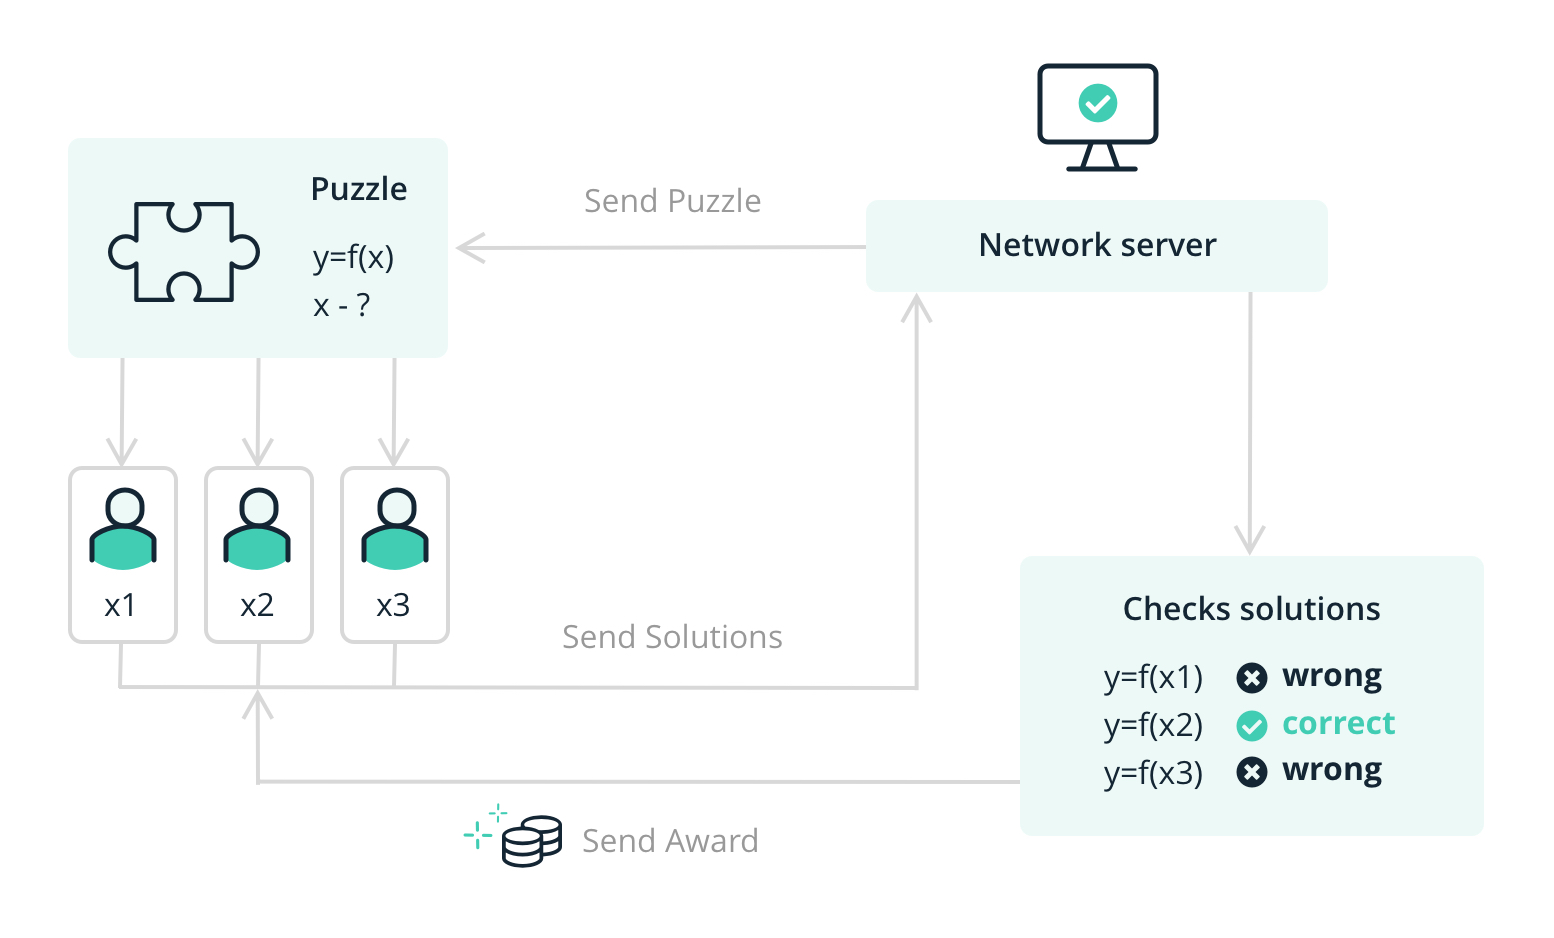
\includegraphics[width=0.7\textwidth]{./Graphics/PoW.png}
            \caption{\textit{PoW}.}
            \label{fig:PoW}
        \end{figure}
    \end{itemize}
    
\

\

    \item \textbf{Proof of Stake (PoS)}:
    \begin{itemize}
        \item Utilizado por \textit{Ethereum 2.0} y otras criptomonedas.
        \item En este modelo, los validadores son seleccionados para crear un nuevo bloque en función de la cantidad de criptomoneda que tienen en "stake" (bloqueada) como garantía. Los validadores reciben recompensas por validar bloques correctamente.
        \item \textit{Eficiencia}: PoS es más eficiente que PoW porque no requiere tanta potencia de cómputo.
        \item \textit{Seguridad}: En teoría, un atacante necesitaría controlar más del 50\% del "stake" total para comprometer la red.
        \begin{figure}[!htbp]
            \centering
            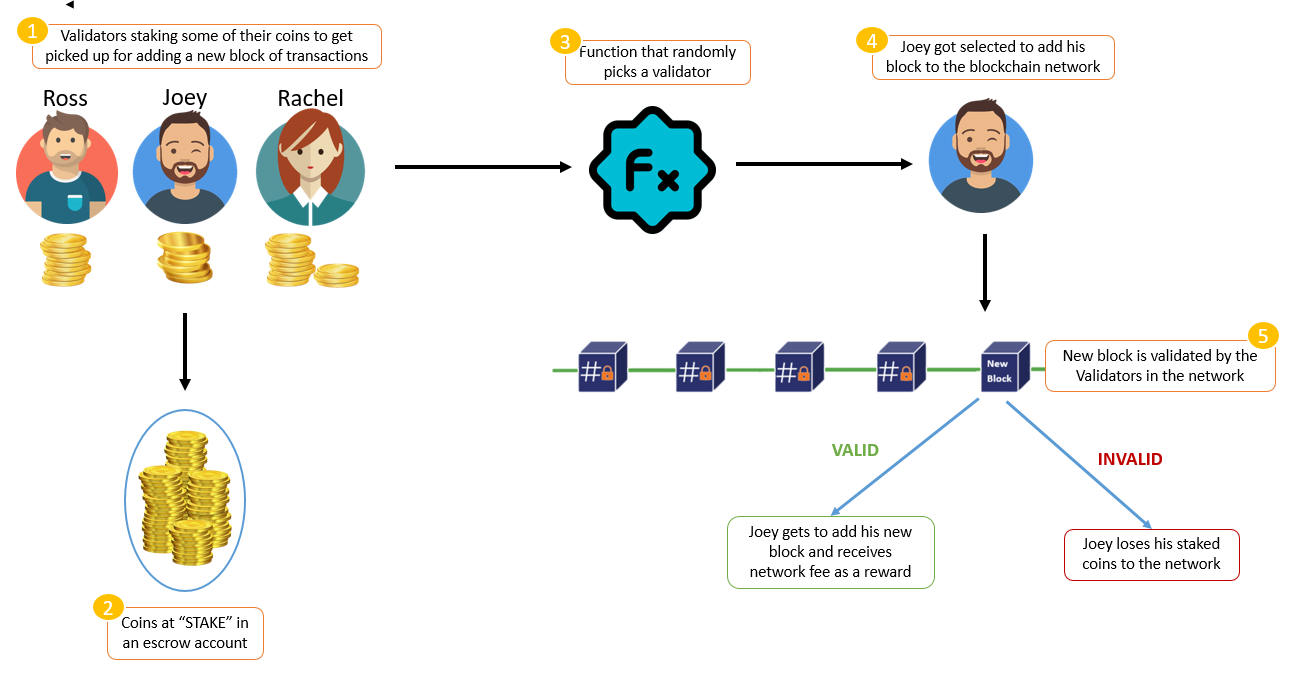
\includegraphics[width=0.7\textwidth]{./Graphics/PoS.png}
            \caption{\textit{PoS}.}
            \label{fig:PoS}
        \end{figure} 
    \end{itemize}

\

\

    \item \textbf{Delegated Proof of Stake (DPoS)}:
    \begin{itemize}
        \item Usado por \textit{EOSIO} \cite{eosio} y otras redes.
        \item Es una versión de PoS donde los participantes votan por representantes (delegados) que validan las transacciones en su nombre. Esto mejora la escalabilidad y eficiencia, pero puede centralizar el poder de validación.
        \begin{figure}[!htbp]
            \centering
            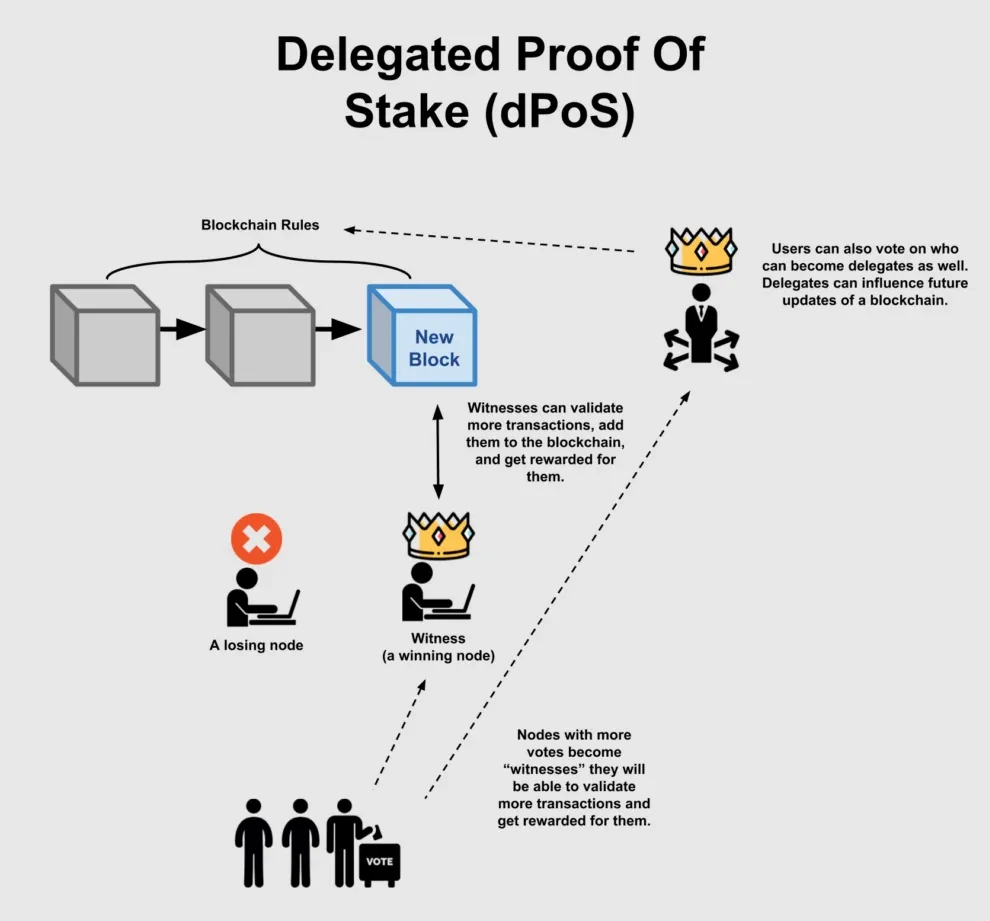
\includegraphics[width=0.5\textwidth]{./Graphics/dPoS.png}
            \caption{\textit{dPoS}.}
            \label{fig:dPoS}
        \end{figure}
    \end{itemize}

\

\

    \item \textbf{Proof of Authority (PoA)}:
    \begin{itemize}
        \item En este sistema, los nodos de validación están predefinidos y son conocidos. Estos nodos son seleccionados con base en su reputación y autoridad.
        \item Usado en redes privadas o de consorcio, donde la confianza en los validadores es clave.
        \begin{figure}[!htbp]
            \centering
            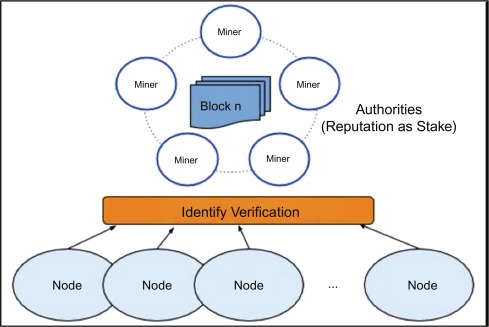
\includegraphics[width=0.7\textwidth]{./Graphics/PoA.png}
            \caption{\textit{PoA}.}
            \label{fig:Po}
        \end{figure}
    \end{itemize}

\end{itemize}

\subsection{Usos y Aplicaciones de Blockchain}

\begin{itemize}
    \item \textbf{Criptomonedas:} Blockchain se usa en Bitcoin, Ethereum y otras criptomonedas para permitir intercambios de valor descentralizados, eliminando intermediarios como los bancos y asegurando transacciones rápidas y económicas.
    
    \item \textbf{Contratos Inteligentes (Smart Contracts):} Programas autoejecutables que se ejecutan cuando se cumplen condiciones predefinidas. Automatización de contratos en bienes raíces, seguros, préstamos, etc.
    
    \item \textbf{Gestión de la Cadena de Suministro:} Rastreabilidad y transparencia de productos a lo largo de la cadena de suministro. Aplicaciones en alimentos, medicamentos y productos de lujo para prevenir fraudes.
        
    \item \textbf{Gobernanza Descentralizada:} Creación de sistemas de gobernanza más transparentes y participativos en organizaciones descentralizadas y autónomas (DAO). Se utiliza en votaciones electrónicas y decisiones colectivas.
    
    \item \textbf{Finanzas Descentralizadas (DeFi):} Plataformas financieras sin intermediarios, como préstamos, seguros, intercambio de activos y DEX. Promueve el ahorro y préstamo en un entorno descentralizado.
    
    \item \textbf{Propiedad Intelectual y Derechos de Autor:} Blockchain gestiona los derechos de autor y permite la tokenización de activos digitales como música, arte y coleccionables (NFTs), garantizando una compensación justa a los creadores.
    
    \item \textbf{Sector Salud:} Blockchain mejora la gestión de registros médicos electrónicos y rastrea la cadena de suministro de medicamentos, evitando falsificaciones y mejorando la calidad del servicio.
    
    \item \textbf{Energía y Sostenibilidad:} Facilita redes de energía descentralizadas donde los usuarios venden y compran energía renovable. También permite el rastreo de huella de carbono en empresas y gobiernos.
    
    \item \textbf{Votación Electrónica:} Proporciona un sistema de votación seguro, transparente y verificable, garantizando la integridad de los votos y previniendo fraudes electorales.
    
    \item \textbf{Tokenización de Activos:} Transformación de activos físicos o digitales en tokens que se pueden negociar, aplicable a inmuebles, activos financieros y productos de lujo.
    
    \item \textbf{Redes Sociales Descentralizadas:} Plataformas donde los usuarios mantienen el control sobre sus datos y contenido, protegiendo la privacidad y eliminando intermediarios.
\end{itemize}

\section{Hyperledger Fabric}
\subsubsection{Canales y Nodos en Hyperledger Fabric}

A diferencia de otras blockchains públicas donde todas las transacciones son visibles para todos los participantes, Hyperledger Fabric introduce el concepto de \textbf{canales}\cite{hyperledgerfabric}.

\begin{itemize}
    \item Un \textbf{canal} es una subred dentro de la blockchain donde un conjunto específico de participantes puede comunicarse de manera privada.
    \item Cada canal es gestionado por nodos llamados \textbf{Orderers}, los cuales tienen la función de organizar las transacciones en bloques y distribuirlos a los nodos validadores (peers).
    \item Los canales pueden ser configurados para que solo ciertas organizaciones tengan acceso a los datos y transacciones dentro de ellos.
\end{itemize}

\subsubsection{Estructura de Organizaciones y Peers}

Hyperledger Fabric permite la participación de múltiples \textbf{organizaciones}\cite{hyperledgerfabric}, cada una con su propio conjunto de nodos llamados \textbf{Peers}.

\begin{itemize}
    \item \textbf{Peers:} Son los nodos que mantienen la información del ledger y ejecutan los contratos inteligentes (chaincodes).
    \item \textbf{Organizaciones:} Son entidades dentro de la red que administran sus propios peers y participan en la toma de decisiones sobre la gestión del canal.
    \item \textbf{Endorsing Peers:} Son aquellos que validan y ejecutan transacciones antes de que sean enviadas a los orderers para su inclusión en un bloque.
    \item \textbf{Anchor Peer:} Son nodos dentro de una organización que facilita la comunicación entre distintas organizaciones en un canal. Sirve como punto de referencia para compartir información sobre la topología de la red y permite que los peers de diferentes organizaciones se descubran entre sí sin necesidad de conexión directa.
\end{itemize}


\begin{figure}[!htbp]
    \centering
    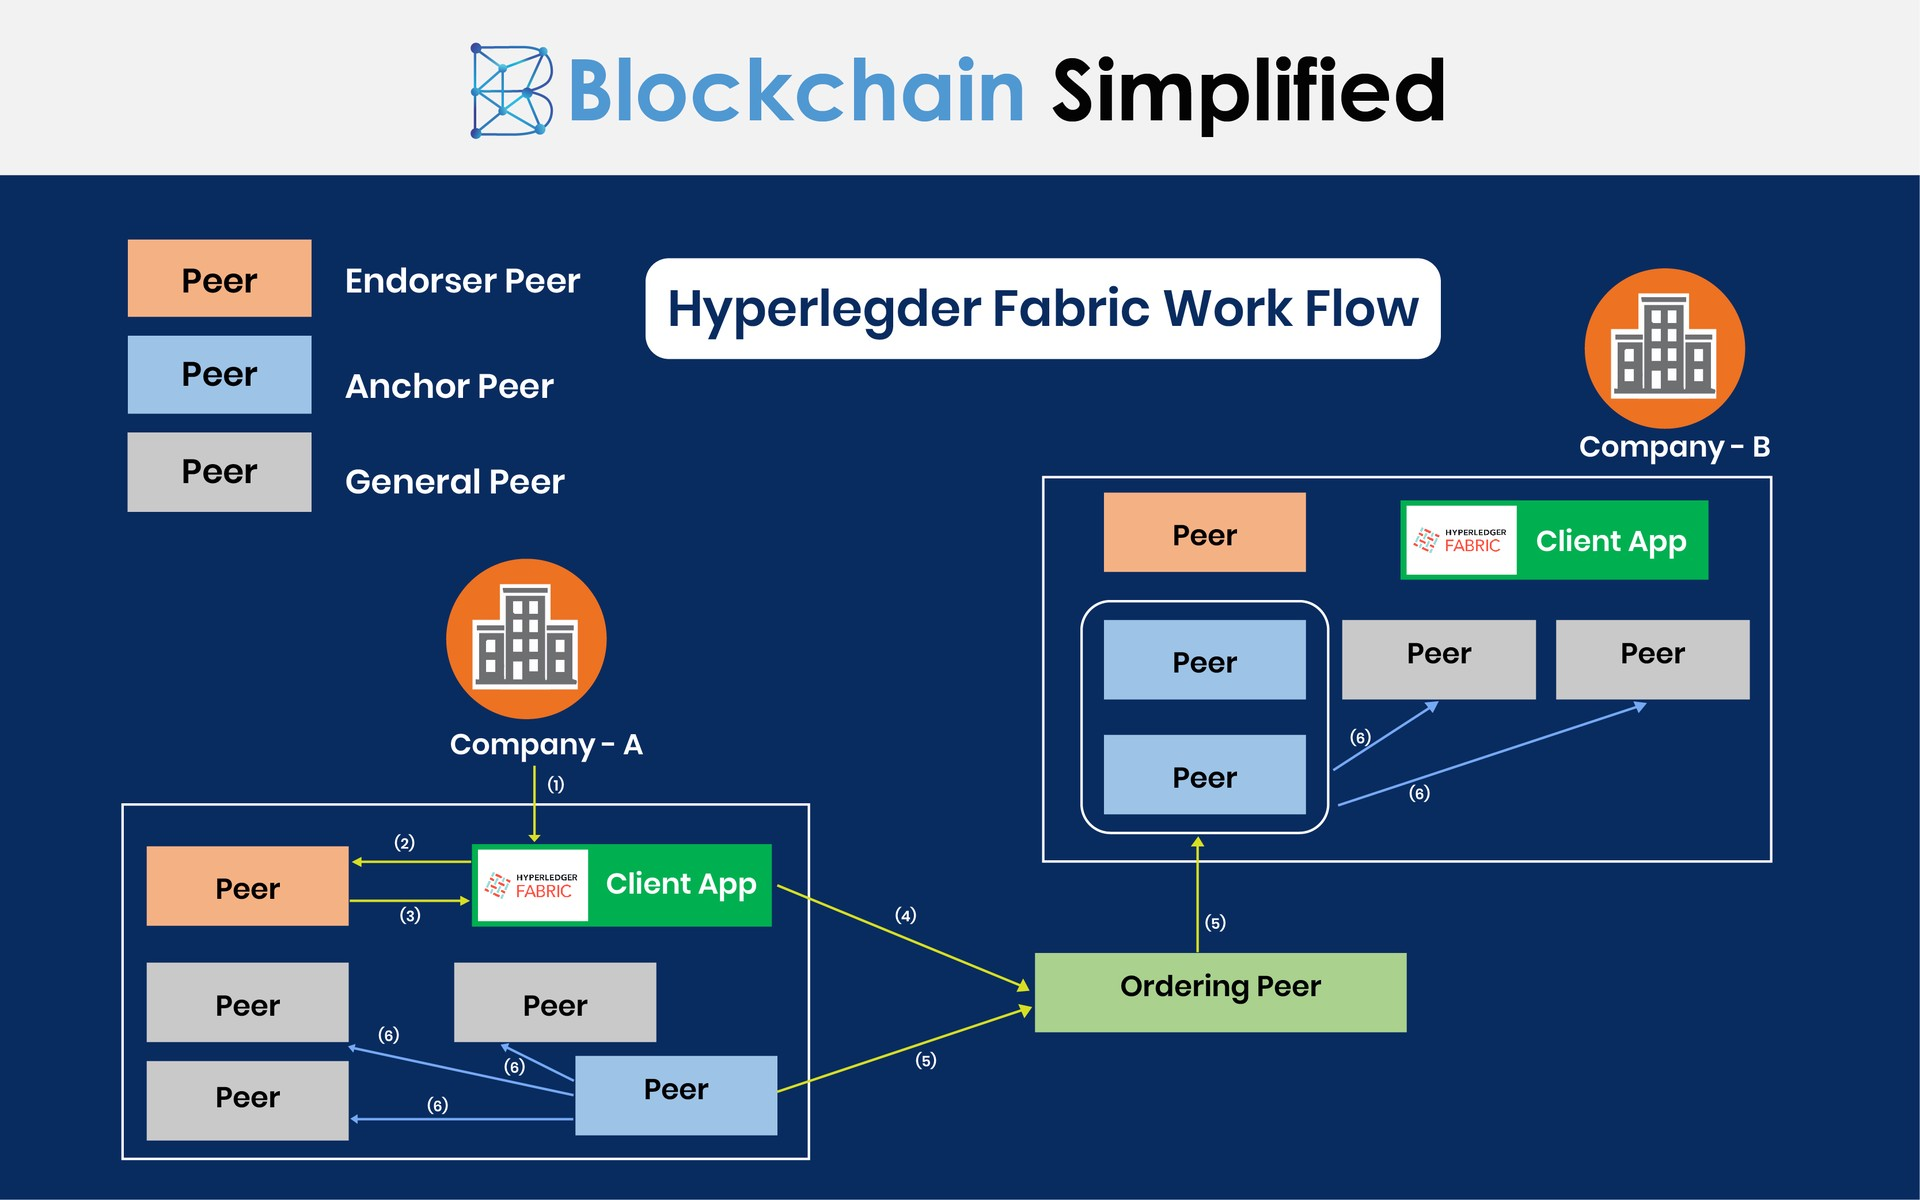
\includegraphics[width=0.7\textwidth]{./Graphics/HLF.png}
    \caption{\textit{Hyperledger Fabric}.}
    \label{fig:HLF}
\end{figure}